\documentclass[]{article}
\usepackage{lmodern}
\usepackage{amssymb,amsmath}
\usepackage{ifxetex,ifluatex}
\usepackage{fixltx2e} % provides \textsubscript
\ifnum 0\ifxetex 1\fi\ifluatex 1\fi=0 % if pdftex
  \usepackage[T1]{fontenc}
  \usepackage[utf8]{inputenc}
\else % if luatex or xelatex
  \ifxetex
    \usepackage{mathspec}
  \else
    \usepackage{fontspec}
  \fi
  \defaultfontfeatures{Ligatures=TeX,Scale=MatchLowercase}
\fi
% use upquote if available, for straight quotes in verbatim environments
\IfFileExists{upquote.sty}{\usepackage{upquote}}{}
% use microtype if available
\IfFileExists{microtype.sty}{%
\usepackage{microtype}
\UseMicrotypeSet[protrusion]{basicmath} % disable protrusion for tt fonts
}{}
\usepackage[margin=1in]{geometry}
\usepackage{hyperref}
\hypersetup{unicode=true,
            pdftitle={Curs Biostatistica 2017 - Laborator 1 \& 2},
            pdfborder={0 0 0},
            breaklinks=true}
\urlstyle{same}  % don't use monospace font for urls
\usepackage{color}
\usepackage{fancyvrb}
\newcommand{\VerbBar}{|}
\newcommand{\VERB}{\Verb[commandchars=\\\{\}]}
\DefineVerbatimEnvironment{Highlighting}{Verbatim}{commandchars=\\\{\}}
% Add ',fontsize=\small' for more characters per line
\usepackage{framed}
\definecolor{shadecolor}{RGB}{248,248,248}
\newenvironment{Shaded}{\begin{snugshade}}{\end{snugshade}}
\newcommand{\KeywordTok}[1]{\textcolor[rgb]{0.13,0.29,0.53}{\textbf{{#1}}}}
\newcommand{\DataTypeTok}[1]{\textcolor[rgb]{0.13,0.29,0.53}{{#1}}}
\newcommand{\DecValTok}[1]{\textcolor[rgb]{0.00,0.00,0.81}{{#1}}}
\newcommand{\BaseNTok}[1]{\textcolor[rgb]{0.00,0.00,0.81}{{#1}}}
\newcommand{\FloatTok}[1]{\textcolor[rgb]{0.00,0.00,0.81}{{#1}}}
\newcommand{\ConstantTok}[1]{\textcolor[rgb]{0.00,0.00,0.00}{{#1}}}
\newcommand{\CharTok}[1]{\textcolor[rgb]{0.31,0.60,0.02}{{#1}}}
\newcommand{\SpecialCharTok}[1]{\textcolor[rgb]{0.00,0.00,0.00}{{#1}}}
\newcommand{\StringTok}[1]{\textcolor[rgb]{0.31,0.60,0.02}{{#1}}}
\newcommand{\VerbatimStringTok}[1]{\textcolor[rgb]{0.31,0.60,0.02}{{#1}}}
\newcommand{\SpecialStringTok}[1]{\textcolor[rgb]{0.31,0.60,0.02}{{#1}}}
\newcommand{\ImportTok}[1]{{#1}}
\newcommand{\CommentTok}[1]{\textcolor[rgb]{0.56,0.35,0.01}{\textit{{#1}}}}
\newcommand{\DocumentationTok}[1]{\textcolor[rgb]{0.56,0.35,0.01}{\textbf{\textit{{#1}}}}}
\newcommand{\AnnotationTok}[1]{\textcolor[rgb]{0.56,0.35,0.01}{\textbf{\textit{{#1}}}}}
\newcommand{\CommentVarTok}[1]{\textcolor[rgb]{0.56,0.35,0.01}{\textbf{\textit{{#1}}}}}
\newcommand{\OtherTok}[1]{\textcolor[rgb]{0.56,0.35,0.01}{{#1}}}
\newcommand{\FunctionTok}[1]{\textcolor[rgb]{0.00,0.00,0.00}{{#1}}}
\newcommand{\VariableTok}[1]{\textcolor[rgb]{0.00,0.00,0.00}{{#1}}}
\newcommand{\ControlFlowTok}[1]{\textcolor[rgb]{0.13,0.29,0.53}{\textbf{{#1}}}}
\newcommand{\OperatorTok}[1]{\textcolor[rgb]{0.81,0.36,0.00}{\textbf{{#1}}}}
\newcommand{\BuiltInTok}[1]{{#1}}
\newcommand{\ExtensionTok}[1]{{#1}}
\newcommand{\PreprocessorTok}[1]{\textcolor[rgb]{0.56,0.35,0.01}{\textit{{#1}}}}
\newcommand{\AttributeTok}[1]{\textcolor[rgb]{0.77,0.63,0.00}{{#1}}}
\newcommand{\RegionMarkerTok}[1]{{#1}}
\newcommand{\InformationTok}[1]{\textcolor[rgb]{0.56,0.35,0.01}{\textbf{\textit{{#1}}}}}
\newcommand{\WarningTok}[1]{\textcolor[rgb]{0.56,0.35,0.01}{\textbf{\textit{{#1}}}}}
\newcommand{\AlertTok}[1]{\textcolor[rgb]{0.94,0.16,0.16}{{#1}}}
\newcommand{\ErrorTok}[1]{\textcolor[rgb]{0.64,0.00,0.00}{\textbf{{#1}}}}
\newcommand{\NormalTok}[1]{{#1}}
\usepackage{graphicx,grffile}
\makeatletter
\def\maxwidth{\ifdim\Gin@nat@width>\linewidth\linewidth\else\Gin@nat@width\fi}
\def\maxheight{\ifdim\Gin@nat@height>\textheight\textheight\else\Gin@nat@height\fi}
\makeatother
% Scale images if necessary, so that they will not overflow the page
% margins by default, and it is still possible to overwrite the defaults
% using explicit options in \includegraphics[width, height, ...]{}
\setkeys{Gin}{width=\maxwidth,height=\maxheight,keepaspectratio}
\IfFileExists{parskip.sty}{%
\usepackage{parskip}
}{% else
\setlength{\parindent}{0pt}
\setlength{\parskip}{6pt plus 2pt minus 1pt}
}
\setlength{\emergencystretch}{3em}  % prevent overfull lines
\providecommand{\tightlist}{%
  \setlength{\itemsep}{0pt}\setlength{\parskip}{0pt}}
\setcounter{secnumdepth}{5}
% Redefines (sub)paragraphs to behave more like sections
\ifx\paragraph\undefined\else
\let\oldparagraph\paragraph
\renewcommand{\paragraph}[1]{\oldparagraph{#1}\mbox{}}
\fi
\ifx\subparagraph\undefined\else
\let\oldsubparagraph\subparagraph
\renewcommand{\subparagraph}[1]{\oldsubparagraph{#1}\mbox{}}
\fi

%%% Use protect on footnotes to avoid problems with footnotes in titles
\let\rmarkdownfootnote\footnote%
\def\footnote{\protect\rmarkdownfootnote}

%%% Change title format to be more compact
\usepackage{titling}

% Create subtitle command for use in maketitle
\newcommand{\subtitle}[1]{
  \posttitle{
    \begin{center}\large#1\end{center}
    }
}

\setlength{\droptitle}{-2em}
  \title{Curs Biostatistica 2017 - Laborator 1 \& 2}
  \pretitle{\vspace{\droptitle}\centering\huge}
  \posttitle{\par}
  \author{}
  \preauthor{}\postauthor{}
  \date{}
  \predate{}\postdate{}

\usepackage{booktabs}
\usepackage{longtable}
\usepackage{framed,color}
\definecolor{shadecolor}{RGB}{248,248,248}

\ifxetex
  \usepackage{letltxmacro}
  \setlength{\XeTeXLinkMargin}{1pt}
  \LetLtxMacro\SavedIncludeGraphics\includegraphics
  \def\includegraphics#1#{% #1 catches optional stuff (star/opt. arg.)
    \IncludeGraphicsAux{#1}%
  }%
  \newcommand*{\IncludeGraphicsAux}[2]{%
    \XeTeXLinkBox{%
      \SavedIncludeGraphics#1{#2}%
    }%
  }%
\fi

\newenvironment{rmdblock}[1]
  {\begin{shaded*}
  \begin{itemize}
  \renewcommand{\labelitemi}{
    \raisebox{-.7\height}[0pt][0pt]{
      {\setkeys{Gin}{width=2em,keepaspectratio}\includegraphics{images/icons/#1}}
    }
  }
  \item
  }
  {
  \end{itemize}
  \end{shaded*}
  }
\newenvironment{rmdcaution}
  {\begin{rmdblock}{caution}}
  {\end{rmdblock}}
\newenvironment{rmdinsight}
  {\begin{rmdblock}{insight}}
  {\end{rmdblock}}
\newenvironment{rmdexercise}
  {\begin{rmdblock}{exercise}}
  {\end{rmdblock}}
\newenvironment{rmdtip}
  {\begin{rmdblock}{tip}}
  {\end{rmdblock}}

\begin{document}
\maketitle

{
\setcounter{tocdepth}{2}
\tableofcontents
}
\section{Intervale de încredere}\label{intervale-de-incredere}

\begin{center}\rule{0.5\linewidth}{\linethickness}\end{center}

\subsection{Densitatea normală}\label{densitatea-normala}

\begin{Shaded}
\begin{Highlighting}[]
\KeywordTok{par}\NormalTok{(}\DataTypeTok{bty=}\StringTok{"n"}\NormalTok{)}
\NormalTok{x <-}\StringTok{ }\KeywordTok{seq}\NormalTok{(-}\DecValTok{4}\NormalTok{,}\DecValTok{4}\NormalTok{,}\DataTypeTok{length=}\DecValTok{501}\NormalTok{)}
\KeywordTok{plot}\NormalTok{(x,}\KeywordTok{dnorm}\NormalTok{(x),}\DataTypeTok{type=}\StringTok{"l"}\NormalTok{,}\DataTypeTok{xaxt=}\StringTok{"n"}\NormalTok{,}\DataTypeTok{yaxt=}\StringTok{"n"}\NormalTok{,}\DataTypeTok{xlab=}\StringTok{""}\NormalTok{,}\DataTypeTok{ylab=}\StringTok{""}\NormalTok{,}\DataTypeTok{lwd=}\DecValTok{2}\NormalTok{)}
\KeywordTok{abline}\NormalTok{(}\DataTypeTok{h=}\DecValTok{0}\NormalTok{)}
\NormalTok{x <-}\StringTok{ }\KeywordTok{c}\NormalTok{(-}\DecValTok{2}\NormalTok{,-}\DecValTok{1}\NormalTok{,}\DecValTok{1}\NormalTok{,}\DecValTok{2}\NormalTok{)}
\KeywordTok{segments}\NormalTok{(x,}\DecValTok{0}\NormalTok{,x,-}\FloatTok{0.01}\NormalTok{,}\DataTypeTok{xpd=}\OtherTok{TRUE}\NormalTok{)}
\KeywordTok{segments}\NormalTok{(}\DecValTok{0}\NormalTok{,}\DecValTok{0}\NormalTok{,}\DecValTok{0}\NormalTok{,-}\FloatTok{0.01}\NormalTok{,}\DataTypeTok{xpd=}\OtherTok{TRUE}\NormalTok{,}\DataTypeTok{col=}\StringTok{"darkgray"}\NormalTok{)}
\KeywordTok{text}\NormalTok{(}\DecValTok{0}\NormalTok{,-}\FloatTok{0.04}\NormalTok{,}\KeywordTok{expression}\NormalTok{(mu),}\DataTypeTok{xpd=}\OtherTok{TRUE}\NormalTok{,}\DataTypeTok{cex=}\FloatTok{1.3}\NormalTok{,}\DataTypeTok{col=}\StringTok{"darkgray"}\NormalTok{)}
\KeywordTok{segments}\NormalTok{(}\KeywordTok{c}\NormalTok{(}\DecValTok{0}\NormalTok{,}\DecValTok{0}\NormalTok{,}\DecValTok{1}\NormalTok{),}\KeywordTok{c}\NormalTok{(}\FloatTok{0.04}\NormalTok{,}\FloatTok{0.03}\NormalTok{,}\FloatTok{0.03}\NormalTok{),}\KeywordTok{c}\NormalTok{(}\DecValTok{1}\NormalTok{,}\DecValTok{0}\NormalTok{,}\DecValTok{1}\NormalTok{),}\KeywordTok{c}\NormalTok{(}\FloatTok{0.04}\NormalTok{,}\FloatTok{0.05}\NormalTok{,}\FloatTok{0.05}\NormalTok{),}\DataTypeTok{lwd=}\DecValTok{2}\NormalTok{,}\DataTypeTok{col=}\StringTok{"brown3"}\NormalTok{)}
\KeywordTok{text}\NormalTok{(}\FloatTok{0.5}\NormalTok{,}\FloatTok{0.07}\NormalTok{,}\KeywordTok{expression}\NormalTok{(sigma/}\KeywordTok{sqrt}\NormalTok{(n)),}\DataTypeTok{cex=}\FloatTok{1.3}\NormalTok{,}\DataTypeTok{col=}\StringTok{"brown3"}\NormalTok{)}
\end{Highlighting}
\end{Shaded}

\begin{center}\includegraphics{Lab_1_2_files/figure-latex/unnamed-chunk-1-1} \end{center}

\subsection{Intervale de încredere pentru
medie}\label{intervale-de-incredere-pentru-medie}

Generarea intervalelor de încredere:

\begin{Shaded}
\begin{Highlighting}[]
\NormalTok{p <-}\StringTok{ }\DecValTok{5}
\NormalTok{n <-}\StringTok{ }\DecValTok{20}

\NormalTok{lo3 <-}\StringTok{ }\NormalTok{hi3 <-}\StringTok{ }\NormalTok{lo2 <-}\StringTok{ }\NormalTok{hi2 <-}\StringTok{ }\NormalTok{lo <-}\StringTok{ }\NormalTok{hi <-}\StringTok{ }\KeywordTok{vector}\NormalTok{(}\StringTok{"list"}\NormalTok{,p)}

\NormalTok{for(i in }\DecValTok{1}\NormalTok{:p) \{}
  \NormalTok{dat <-}\StringTok{ }\KeywordTok{matrix}\NormalTok{(}\KeywordTok{rnorm}\NormalTok{(n*}\DecValTok{10}\NormalTok{,}\FloatTok{3.5}\NormalTok{,}\DataTypeTok{sd=}\FloatTok{1.5}\NormalTok{),}\DataTypeTok{ncol=}\DecValTok{10}\NormalTok{)}
  
  \NormalTok{m <-}\StringTok{ }\KeywordTok{apply}\NormalTok{(dat,}\DecValTok{1}\NormalTok{,mean)}
  \NormalTok{s <-}\StringTok{ }\KeywordTok{apply}\NormalTok{(dat,}\DecValTok{1}\NormalTok{,sd)}
  
  \NormalTok{lo[[i]] <-}\StringTok{ }\NormalTok{m-}\KeywordTok{qnorm}\NormalTok{(}\FloatTok{0.975}\NormalTok{)*}\FloatTok{1.5}\NormalTok{/}\KeywordTok{sqrt}\NormalTok{(}\DecValTok{10}\NormalTok{)}
  \NormalTok{hi[[i]] <-}\StringTok{ }\NormalTok{m+}\KeywordTok{qnorm}\NormalTok{(}\FloatTok{0.975}\NormalTok{)*}\FloatTok{1.5}\NormalTok{/}\KeywordTok{sqrt}\NormalTok{(}\DecValTok{10}\NormalTok{)}
  
  \NormalTok{lo2[[i]] <-}\StringTok{ }\NormalTok{m-}\KeywordTok{qnorm}\NormalTok{(}\FloatTok{0.975}\NormalTok{)*s/}\KeywordTok{sqrt}\NormalTok{(}\DecValTok{10}\NormalTok{)}
  \NormalTok{hi2[[i]] <-}\StringTok{ }\NormalTok{m+}\KeywordTok{qnorm}\NormalTok{(}\FloatTok{0.975}\NormalTok{)*s/}\KeywordTok{sqrt}\NormalTok{(}\DecValTok{10}\NormalTok{)}
  
  \NormalTok{lo3[[i]] <-}\StringTok{ }\NormalTok{m-}\KeywordTok{qt}\NormalTok{(}\FloatTok{0.975}\NormalTok{,}\DecValTok{9}\NormalTok{)*s/}\KeywordTok{sqrt}\NormalTok{(}\DecValTok{10}\NormalTok{)}
  \NormalTok{hi3[[i]] <-}\StringTok{ }\NormalTok{m+}\KeywordTok{qt}\NormalTok{(}\FloatTok{0.975}\NormalTok{,}\DecValTok{9}\NormalTok{)*s/}\KeywordTok{sqrt}\NormalTok{(}\DecValTok{10}\NormalTok{)}
\NormalTok{\}}
\end{Highlighting}
\end{Shaded}

Intervale de încredere atunci când \(\sigma\) este cunoscut:

\begin{Shaded}
\begin{Highlighting}[]
\NormalTok{r <-}\StringTok{ }\KeywordTok{range}\NormalTok{(}\KeywordTok{unlist}\NormalTok{(}\KeywordTok{c}\NormalTok{(lo,hi,lo2,hi2,lo3,hi3)))}

\KeywordTok{par}\NormalTok{(}\DataTypeTok{mfrow=}\KeywordTok{c}\NormalTok{(}\DecValTok{1}\NormalTok{,}\DecValTok{5}\NormalTok{), }\DataTypeTok{las=}\DecValTok{1}\NormalTok{, }\DataTypeTok{mar=}\KeywordTok{c}\NormalTok{(}\FloatTok{5.1}\NormalTok{,}\FloatTok{2.1}\NormalTok{,}\FloatTok{6.1}\NormalTok{,}\FloatTok{2.1}\NormalTok{))}

\NormalTok{for(i in }\DecValTok{1}\NormalTok{:p) \{}
  \KeywordTok{plot}\NormalTok{(}\DecValTok{0}\NormalTok{,}\DecValTok{0}\NormalTok{,}\DataTypeTok{type=}\StringTok{"n"}\NormalTok{,}\DataTypeTok{ylim=}\FloatTok{0.5}\NormalTok{+}\KeywordTok{c}\NormalTok{(}\DecValTok{0}\NormalTok{,n),}\DataTypeTok{xlim=}\NormalTok{r,}\DataTypeTok{ylab=}\StringTok{""}\NormalTok{,}\DataTypeTok{xlab=}\StringTok{""}\NormalTok{,}\DataTypeTok{yaxt=}\StringTok{"n"}\NormalTok{)}
  
  \KeywordTok{abline}\NormalTok{(}\DataTypeTok{v=}\FloatTok{3.5}\NormalTok{,}\DataTypeTok{lty=}\DecValTok{2}\NormalTok{,}\DataTypeTok{col=}\StringTok{"brown3"}\NormalTok{,}\DataTypeTok{lwd=}\DecValTok{2}\NormalTok{)}
  
  \KeywordTok{segments}\NormalTok{(lo[[i]],}\DecValTok{1}\NormalTok{:n,hi[[i]],}\DecValTok{1}\NormalTok{:n,}\DataTypeTok{lwd=}\DecValTok{2}\NormalTok{)}
  
  \NormalTok{o <-}\StringTok{ }\NormalTok{(}\DecValTok{1}\NormalTok{:n)[lo[[i]] >}\StringTok{ }\FloatTok{3.5} \NormalTok{|}\StringTok{ }\NormalTok{hi[[i]] <}\StringTok{ }\FloatTok{3.5}\NormalTok{]}
  
  \KeywordTok{segments}\NormalTok{(lo[[i]][o],o,hi[[i]][o],o,}\DataTypeTok{lwd=}\DecValTok{2}\NormalTok{,}\DataTypeTok{col=}\StringTok{"orange"}\NormalTok{)}
\NormalTok{\}}

\KeywordTok{par}\NormalTok{(}\DataTypeTok{mfrow=}\KeywordTok{c}\NormalTok{(}\DecValTok{1}\NormalTok{,}\DecValTok{1}\NormalTok{))}

\KeywordTok{mtext}\NormalTok{(}\KeywordTok{expression}\NormalTok{(}\KeywordTok{paste}\NormalTok{(}\StringTok{"100 intervale de încredere pentru "}\NormalTok{,mu)),}
      \DataTypeTok{side=}\DecValTok{3}\NormalTok{,}\DataTypeTok{cex=}\FloatTok{1.5}\NormalTok{,}\DataTypeTok{xpd=}\OtherTok{TRUE}\NormalTok{,}\DataTypeTok{line=}\DecValTok{4}\NormalTok{)}
\KeywordTok{mtext}\NormalTok{(}\KeywordTok{expression}\NormalTok{(}\KeywordTok{paste}\NormalTok{(}\StringTok{"("}\NormalTok{,sigma,}\StringTok{" cunoscut)"}\NormalTok{)),}\DataTypeTok{side=}\DecValTok{3}\NormalTok{,}\DataTypeTok{cex=}\FloatTok{1.3}\NormalTok{,}
      \DataTypeTok{xpd=}\OtherTok{TRUE}\NormalTok{,}\DataTypeTok{line=}\FloatTok{2.7}\NormalTok{)}
\end{Highlighting}
\end{Shaded}

\begin{center}\includegraphics[width=0.9\linewidth]{Lab_1_2_files/figure-latex/unnamed-chunk-3-1} \end{center}

Intervale de încredere \textbf{incorecte} atunci când \(\sigma\) nu este
cunoscut:

\begin{Shaded}
\begin{Highlighting}[]
\KeywordTok{par}\NormalTok{(}\DataTypeTok{mfrow=}\KeywordTok{c}\NormalTok{(}\DecValTok{1}\NormalTok{,}\DecValTok{5}\NormalTok{), }\DataTypeTok{las=}\DecValTok{1}\NormalTok{, }\DataTypeTok{mar=}\KeywordTok{c}\NormalTok{(}\FloatTok{5.1}\NormalTok{,}\FloatTok{2.1}\NormalTok{,}\FloatTok{6.1}\NormalTok{,}\FloatTok{2.1}\NormalTok{))}
\NormalTok{for(i in }\DecValTok{1}\NormalTok{:p) \{}
  \KeywordTok{plot}\NormalTok{(}\DecValTok{0}\NormalTok{,}\DecValTok{0}\NormalTok{,}\DataTypeTok{type=}\StringTok{"n"}\NormalTok{,}\DataTypeTok{ylim=}\FloatTok{0.5}\NormalTok{+}\KeywordTok{c}\NormalTok{(}\DecValTok{0}\NormalTok{,n),}\DataTypeTok{xlim=}\NormalTok{r,}\DataTypeTok{ylab=}\StringTok{""}\NormalTok{,}\DataTypeTok{xlab=}\StringTok{""}\NormalTok{,}\DataTypeTok{yaxt=}\StringTok{"n"}\NormalTok{)}
  \KeywordTok{abline}\NormalTok{(}\DataTypeTok{v=}\FloatTok{3.5}\NormalTok{,}\DataTypeTok{lty=}\DecValTok{2}\NormalTok{,}\DataTypeTok{col=}\StringTok{"brown3"}\NormalTok{,}\DataTypeTok{lwd=}\DecValTok{2}\NormalTok{)}
  \KeywordTok{segments}\NormalTok{(lo2[[i]],}\DecValTok{1}\NormalTok{:n,hi2[[i]],}\DecValTok{1}\NormalTok{:n,}\DataTypeTok{lwd=}\DecValTok{2}\NormalTok{)}
  \NormalTok{o <-}\StringTok{ }\NormalTok{(}\DecValTok{1}\NormalTok{:n)[lo2[[i]] >}\StringTok{ }\FloatTok{3.5} \NormalTok{|}\StringTok{ }\NormalTok{hi2[[i]] <}\StringTok{ }\FloatTok{3.5}\NormalTok{]}
  \KeywordTok{segments}\NormalTok{(lo2[[i]][o],o,hi2[[i]][o],o,}\DataTypeTok{lwd=}\DecValTok{2}\NormalTok{,}\DataTypeTok{col=}\StringTok{"orange"}\NormalTok{)}
\NormalTok{\}}
\KeywordTok{par}\NormalTok{(}\DataTypeTok{mfrow=}\KeywordTok{c}\NormalTok{(}\DecValTok{1}\NormalTok{,}\DecValTok{1}\NormalTok{))}
\KeywordTok{mtext}\NormalTok{(}\KeywordTok{expression}\NormalTok{(}\KeywordTok{paste}\NormalTok{(}\StringTok{"100 intervale de încredere incorecte pentru "}\NormalTok{,mu)),}\DataTypeTok{side=}\DecValTok{3}\NormalTok{,}\DataTypeTok{cex=}\FloatTok{1.5}\NormalTok{,}\DataTypeTok{xpd=}\OtherTok{TRUE}\NormalTok{,}\DataTypeTok{line=}\DecValTok{4}\NormalTok{)}
\KeywordTok{mtext}\NormalTok{(}\KeywordTok{expression}\NormalTok{(}\KeywordTok{paste}\NormalTok{(}\StringTok{"("}\NormalTok{,sigma,}\StringTok{" necunoscut)"}\NormalTok{)),}
      \DataTypeTok{side=}\DecValTok{3}\NormalTok{,}\DataTypeTok{cex=}\FloatTok{1.3}\NormalTok{,}\DataTypeTok{xpd=}\OtherTok{TRUE}\NormalTok{,}\DataTypeTok{line=}\FloatTok{2.7}\NormalTok{)}
\end{Highlighting}
\end{Shaded}

\begin{center}\includegraphics[width=0.9\linewidth]{Lab_1_2_files/figure-latex/unnamed-chunk-4-1} \end{center}

Intervale de încredere \textbf{corecte} atunci când \(\sigma\) nu este
cunoscut:

\begin{Shaded}
\begin{Highlighting}[]
\KeywordTok{par}\NormalTok{(}\DataTypeTok{mfrow=}\KeywordTok{c}\NormalTok{(}\DecValTok{1}\NormalTok{,}\DecValTok{5}\NormalTok{), }\DataTypeTok{las=}\DecValTok{1}\NormalTok{, }\DataTypeTok{mar=}\KeywordTok{c}\NormalTok{(}\FloatTok{5.1}\NormalTok{,}\FloatTok{2.1}\NormalTok{,}\FloatTok{6.1}\NormalTok{,}\FloatTok{2.1}\NormalTok{))}
\NormalTok{for(i in }\DecValTok{1}\NormalTok{:p) \{}
  \KeywordTok{plot}\NormalTok{(}\DecValTok{0}\NormalTok{,}\DecValTok{0}\NormalTok{,}\DataTypeTok{type=}\StringTok{"n"}\NormalTok{,}\DataTypeTok{ylim=}\FloatTok{0.5}\NormalTok{+}\KeywordTok{c}\NormalTok{(}\DecValTok{0}\NormalTok{,n),}\DataTypeTok{xlim=}\NormalTok{r,}\DataTypeTok{ylab=}\StringTok{""}\NormalTok{,}\DataTypeTok{xlab=}\StringTok{""}\NormalTok{,}\DataTypeTok{yaxt=}\StringTok{"n"}\NormalTok{)}
  \KeywordTok{abline}\NormalTok{(}\DataTypeTok{v=}\FloatTok{3.5}\NormalTok{,}\DataTypeTok{lty=}\DecValTok{2}\NormalTok{,}\DataTypeTok{col=}\StringTok{"brown3"}\NormalTok{,}\DataTypeTok{lwd=}\DecValTok{2}\NormalTok{)}
  \KeywordTok{segments}\NormalTok{(lo3[[i]],}\DecValTok{1}\NormalTok{:n,hi3[[i]],}\DecValTok{1}\NormalTok{:n,}\DataTypeTok{lwd=}\DecValTok{2}\NormalTok{)}
  \NormalTok{o <-}\StringTok{ }\NormalTok{(}\DecValTok{1}\NormalTok{:n)[lo3[[i]] >}\StringTok{ }\FloatTok{3.5} \NormalTok{|}\StringTok{ }\NormalTok{hi3[[i]] <}\StringTok{ }\FloatTok{3.5}\NormalTok{]}
  \KeywordTok{segments}\NormalTok{(lo3[[i]][o],o,hi3[[i]][o],o,}\DataTypeTok{lwd=}\DecValTok{2}\NormalTok{,}\DataTypeTok{col=}\StringTok{"orange"}\NormalTok{)}
\NormalTok{\}}
\KeywordTok{par}\NormalTok{(}\DataTypeTok{mfrow=}\KeywordTok{c}\NormalTok{(}\DecValTok{1}\NormalTok{,}\DecValTok{1}\NormalTok{))}
\KeywordTok{mtext}\NormalTok{(}\KeywordTok{expression}\NormalTok{(}\KeywordTok{paste}\NormalTok{(}\StringTok{"100 intervale de încredere pentru "}\NormalTok{,mu)),}
      \DataTypeTok{side=}\DecValTok{3}\NormalTok{,}\DataTypeTok{cex=}\FloatTok{1.5}\NormalTok{,}\DataTypeTok{xpd=}\OtherTok{TRUE}\NormalTok{,}\DataTypeTok{line=}\DecValTok{4}\NormalTok{)}
\KeywordTok{mtext}\NormalTok{(}\KeywordTok{expression}\NormalTok{(}\KeywordTok{paste}\NormalTok{(}\StringTok{"("}\NormalTok{,sigma,}\StringTok{" necunoscut)"}\NormalTok{)),}
      \DataTypeTok{side=}\DecValTok{3}\NormalTok{,}\DataTypeTok{cex=}\FloatTok{1.3}\NormalTok{,}\DataTypeTok{xpd=}\OtherTok{TRUE}\NormalTok{,}\DataTypeTok{line=}\FloatTok{2.7}\NormalTok{)}
\end{Highlighting}
\end{Shaded}

\begin{center}\includegraphics[width=0.9\linewidth]{Lab_1_2_files/figure-latex/unnamed-chunk-5-1} \end{center}

\section{Testarea ipotezelor statistice: inferență asupra unui
eșantion}\label{testarea-ipotezelor-statistice-inferenta-asupra-unui-esantion}

\begin{center}\rule{0.5\linewidth}{\linethickness}\end{center}

\subsection{Exemplul 1}\label{exemplul-1}

\begin{quote}
Care este temperatura normală a corpului uman ?
(\href{readings/BodyTemp.pdf}{vezi articol}) Ne dorim să testăm din
punct de vedere statistic dacă temperatura medie a corpului uman este de
\(37^\circ C\) plecând de la următorul set de date
\href{data/normtemp.txt}{descarcă} (sursa originală a datelor este
\emph{Mackowiak, P. A., Wasserman, S. S., and Levine, M. M. (1992). A
Critical Appraisal of 98.6 Degrees F, the Upper Limit of the Normal Body
Temperature, and Other Legacies of Carl Reinhold August Wunderlich.
Journal of the American Medical Association, 268, 1578-1580}).
\end{quote}

Pentru a citi datele putem folosi două metode: sau să le citim direct
din pagina de internet (prin comanda \texttt{read.table})

\begin{Shaded}
\begin{Highlighting}[]
\NormalTok{file =}\StringTok{ "https://alexamarioarei.github.io/Teaching/Biostatistics/labs/data/normtemp.txt"}
\NormalTok{normtemp =}\StringTok{ }\KeywordTok{read.table}\NormalTok{(file, }\DataTypeTok{header=}\NormalTok{F, }\DataTypeTok{col.names=}\KeywordTok{c}\NormalTok{(}\StringTok{"temp"}\NormalTok{,}\StringTok{"sex"}\NormalTok{,}\StringTok{"hr"}\NormalTok{))}

\KeywordTok{head}\NormalTok{(normtemp)}
\end{Highlighting}
\end{Shaded}

\begin{verbatim}
##   temp sex hr
## 1 96.3   1 70
## 2 96.7   1 71
## 3 96.9   1 74
## 4 97.0   1 80
## 5 97.1   1 73
## 6 97.1   1 75
\end{verbatim}

sau descărcând local fișierul cu date și înlocuind adresa de internet
din \texttt{file} cu cea locală.

Temperatura apare în grade Fahrenheit și am dori să transformăm în grade
Celsius folosind formula:

\[
  T_C = 5(T_F-32)/9
\]

\begin{Shaded}
\begin{Highlighting}[]
\NormalTok{normtemp$tempC =}\StringTok{ }\NormalTok{(normtemp$temp -}\StringTok{ }\DecValTok{32}\NormalTok{)*}\DecValTok{5}\NormalTok{/}\DecValTok{9} 
\NormalTok{degreesC =}\StringTok{ }\NormalTok{normtemp$tempC}
\end{Highlighting}
\end{Shaded}

Testul t-student presupune că eșantionul (independent) a provenit
dintr-o populație normală și pentru aceasta putem verifica ipoteza de
normalitate (\texttt{QQ\ plot}):

\begin{Shaded}
\begin{Highlighting}[]
\KeywordTok{qqnorm}\NormalTok{(degreesC)}
\KeywordTok{qqline}\NormalTok{(degreesC)}
\end{Highlighting}
\end{Shaded}

\begin{center}\includegraphics[width=0.9\linewidth]{Lab_1_2_files/figure-latex/unnamed-chunk-8-1} \end{center}

Trasăm histograma:

\begin{Shaded}
\begin{Highlighting}[]
\KeywordTok{hist}\NormalTok{(degreesC, }\DataTypeTok{probability =} \NormalTok{T)}
\NormalTok{degM =}\StringTok{ }\KeywordTok{mean}\NormalTok{(degreesC)}
\NormalTok{degSD =}\StringTok{ }\KeywordTok{sd}\NormalTok{(degreesC)}
\KeywordTok{curve}\NormalTok{(}\KeywordTok{dnorm}\NormalTok{(x, degM, degSD), }\DataTypeTok{add =} \NormalTok{T, }\DataTypeTok{col =} \StringTok{"brown3"}\NormalTok{)}
\end{Highlighting}
\end{Shaded}

\begin{center}\includegraphics[width=0.9\linewidth]{Lab_1_2_files/figure-latex/unnamed-chunk-9-1} \end{center}

Trasăm densitatea:

\begin{Shaded}
\begin{Highlighting}[]
\KeywordTok{plot}\NormalTok{(}\KeywordTok{density}\NormalTok{(degreesC))}
\KeywordTok{curve}\NormalTok{(}\KeywordTok{dnorm}\NormalTok{(x, degM, degSD), }\DataTypeTok{add =} \NormalTok{T, }\DataTypeTok{col =} \StringTok{"brown3"}\NormalTok{)}
\end{Highlighting}
\end{Shaded}

\begin{center}\includegraphics[width=0.9\linewidth]{Lab_1_2_files/figure-latex/unnamed-chunk-10-1} \end{center}

Testăm ipoteza de normalitate (folosind testul \texttt{Shapiro-Wilk}):

\begin{Shaded}
\begin{Highlighting}[]
\KeywordTok{shapiro.test}\NormalTok{(degreesC)}\CommentTok{# distributia pare sa fie aproape de normala si testul nu detecteaza }
\end{Highlighting}
\end{Shaded}

\begin{verbatim}
## 
##  Shapiro-Wilk normality test
## 
## data:  degreesC
## W = 0.98658, p-value = 0.2332
\end{verbatim}

\begin{Shaded}
\begin{Highlighting}[]
                      \CommentTok{# o abatere semnificativa fata de normala}
\end{Highlighting}
\end{Shaded}

Distribuția pare să fie aproape de normală, testul Shapiro-Wilk nu
detectează o deviație semnificantă de la normalitate.

\begin{Shaded}
\begin{Highlighting}[]
\KeywordTok{t.test}\NormalTok{(degreesC, }\DataTypeTok{mu =} \DecValTok{37}\NormalTok{, }\DataTypeTok{alternative =} \StringTok{"two.sided"}\NormalTok{) }\CommentTok{# respingem H0}
\end{Highlighting}
\end{Shaded}

\begin{verbatim}
## 
##  One Sample t-test
## 
## data:  degreesC
## t = -5.4548, df = 129, p-value = 2.411e-07
## alternative hypothesis: true mean is not equal to 37
## 95 percent confidence interval:
##  36.73445 36.87581
## sample estimates:
## mean of x 
##  36.80513
\end{verbatim}

\begin{Shaded}
\begin{Highlighting}[]
\NormalTok{ttest_deg =}\StringTok{ }\KeywordTok{t.test}\NormalTok{(degreesC, }\DataTypeTok{mu =} \DecValTok{37}\NormalTok{)}

\NormalTok{ttest_deg$statistic}
\end{Highlighting}
\end{Shaded}

\begin{verbatim}
##         t 
## -5.454823
\end{verbatim}

\begin{Shaded}
\begin{Highlighting}[]
\NormalTok{ttest_deg$p.value}
\end{Highlighting}
\end{Shaded}

\begin{verbatim}
## [1] 2.410632e-07
\end{verbatim}

\begin{Shaded}
\begin{Highlighting}[]
\NormalTok{ttest_deg$conf.int}
\end{Highlighting}
\end{Shaded}

\begin{verbatim}
## [1] 36.73445 36.87581
## attr(,"conf.level")
## [1] 0.95
\end{verbatim}

Dacă nu avem datele și avem o problemă de tipul: un eșantion de 130 de
persoane a fost selectionat și temperatura corpului a fost masurată.
Media eșantionului a fost \texttt{36.805} iar abaterea standard
\texttt{0.4073}. Testati ipoteza nulă că media temperaturii corpului
uman este de \texttt{37} grade Celsius.

În acest caz avem:

\begin{Shaded}
\begin{Highlighting}[]
\NormalTok{t.obt =}\StringTok{ }\NormalTok{(}\FloatTok{36.805} \NormalTok{-}\StringTok{ }\DecValTok{37}\NormalTok{)/(}\FloatTok{0.4073}\NormalTok{/}\KeywordTok{sqrt}\NormalTok{(}\DecValTok{130}\NormalTok{))}
\NormalTok{t.obt}
\end{Highlighting}
\end{Shaded}

\begin{verbatim}
## [1] -5.458733
\end{verbatim}

\begin{Shaded}
\begin{Highlighting}[]
\KeywordTok{qt}\NormalTok{(}\KeywordTok{c}\NormalTok{(}\FloatTok{0.25}\NormalTok{, }\FloatTok{0.975}\NormalTok{), }\DataTypeTok{df =} \DecValTok{129}\NormalTok{) }\CommentTok{# valorile critice pentru alpha = 0.05}
\end{Highlighting}
\end{Shaded}

\begin{verbatim}
## [1] -0.6763963  1.9785245
\end{verbatim}

\begin{Shaded}
\begin{Highlighting}[]
\DecValTok{2}\NormalTok{*}\KeywordTok{pt}\NormalTok{(t.obt, }\DataTypeTok{df =} \DecValTok{129}\NormalTok{) }\CommentTok{# p valoarea pentru testul two-tailed}
\end{Highlighting}
\end{Shaded}

\begin{verbatim}
## [1] 2.367923e-07
\end{verbatim}

Ca să automatizăm aceste calcule putem crea o funcție:

\begin{Shaded}
\begin{Highlighting}[]
\NormalTok{t.single =}\StringTok{ }\NormalTok{function(obs.mean, mu, SD, n) \{}
  \NormalTok{t.obt =}\StringTok{ }\NormalTok{(obs.mean -}\StringTok{ }\NormalTok{mu) /}\StringTok{ }\NormalTok{(SD /}\StringTok{ }\KeywordTok{sqrt}\NormalTok{(n))}
  \NormalTok{p.value =}\StringTok{ }\KeywordTok{pt}\NormalTok{(}\KeywordTok{abs}\NormalTok{(t.obt), }\DataTypeTok{df=}\NormalTok{n}\DecValTok{-1}\NormalTok{, }\DataTypeTok{lower.tail=}\NormalTok{F)}
  \KeywordTok{print}\NormalTok{(}\KeywordTok{c}\NormalTok{(}\DataTypeTok{t.obt =} \NormalTok{t.obt, }\DataTypeTok{p.value =} \NormalTok{p.value))}
  \KeywordTok{warning}\NormalTok{(}\StringTok{"P-value pentru one-sided. Dubleaza pentru two-sided."}\NormalTok{)}
\NormalTok{\}}

\KeywordTok{t.single}\NormalTok{(}\FloatTok{36.805}\NormalTok{, }\DataTypeTok{mu =} \DecValTok{37}\NormalTok{, }\DataTypeTok{SD =} \FloatTok{0.4073}\NormalTok{, }\DataTypeTok{n =} \DecValTok{130}\NormalTok{)}
\end{Highlighting}
\end{Shaded}

\begin{verbatim}
##         t.obt       p.value 
## -5.458733e+00  1.183961e-07
\end{verbatim}

\begin{verbatim}
## Warning in t.single(36.805, mu = 37, SD = 0.4073, n = 130): P-value pentru
## one-sided. Dubleaza pentru two-sided.
\end{verbatim}

\section{Testarea ipotezelor statistice: inferență asupra a două
eșantioane}\label{testarea-ipotezelor-statistice-inferenta-asupra-a-doua-esantioane}

\begin{center}\rule{0.5\linewidth}{\linethickness}\end{center}

\subsection{Exemplul 1}\label{exemplul-1-1}

În contextul exemplului anterior, să presupunem că vrem să vedem dacă
există vreo diferență între temperatura medie la bărbați și temperatura
medie la femei.

\begin{Shaded}
\begin{Highlighting}[]
\KeywordTok{str}\NormalTok{(normtemp)}
\end{Highlighting}
\end{Shaded}

\begin{verbatim}
## 'data.frame':    130 obs. of  4 variables:
##  $ temp : num  96.3 96.7 96.9 97 97.1 97.1 97.1 97.2 97.3 97.4 ...
##  $ sex  : int  1 1 1 1 1 1 1 1 1 1 ...
##  $ hr   : int  70 71 74 80 73 75 82 64 69 70 ...
##  $ tempC: num  35.7 35.9 36.1 36.1 36.2 ...
\end{verbatim}

\begin{Shaded}
\begin{Highlighting}[]
\NormalTok{tempB =}\StringTok{ }\NormalTok{normtemp$tempC[}\KeywordTok{which}\NormalTok{(normtemp$sex ==}\StringTok{ }\DecValTok{1}\NormalTok{)]}
\NormalTok{tempF =}\StringTok{ }\NormalTok{normtemp$tempC[}\KeywordTok{which}\NormalTok{(normtemp$sex ==}\StringTok{ }\DecValTok{2}\NormalTok{)]}
\end{Highlighting}
\end{Shaded}

Ilustrare a temperaturii bărbaților și a femeilor:

\begin{Shaded}
\begin{Highlighting}[]
\KeywordTok{par}\NormalTok{(}\DataTypeTok{mfrow=}\KeywordTok{c}\NormalTok{(}\DecValTok{1}\NormalTok{,}\DecValTok{2}\NormalTok{))}
\KeywordTok{plot}\NormalTok{(}\KeywordTok{density}\NormalTok{(tempB), }\DataTypeTok{main=}\StringTok{"Temperatura Barbatilor"}\NormalTok{)}
\KeywordTok{plot}\NormalTok{(}\KeywordTok{density}\NormalTok{(tempF), }\DataTypeTok{main=}\StringTok{"Temperatura Femeilor"}\NormalTok{)}
\end{Highlighting}
\end{Shaded}

\begin{center}\includegraphics[width=0.9\linewidth]{Lab_1_2_files/figure-latex/unnamed-chunk-17-1} \end{center}

Sub formă de \texttt{boxplot}:

\begin{Shaded}
\begin{Highlighting}[]
\KeywordTok{par}\NormalTok{(}\DataTypeTok{mfrow =} \KeywordTok{c}\NormalTok{(}\DecValTok{1}\NormalTok{,}\DecValTok{1}\NormalTok{))}
\KeywordTok{boxplot}\NormalTok{(tempB, tempF, }\DataTypeTok{ylab=}\StringTok{"Temperatura"}\NormalTok{,     }\CommentTok{# plot and label y-axis}
                \DataTypeTok{names=}\KeywordTok{c}\NormalTok{(}\StringTok{"Barbati"}\NormalTok{,}\StringTok{"Femei"}\NormalTok{),   }\CommentTok{# group names on x-axis}
                \DataTypeTok{main=}\StringTok{"Temperatura in functie de sex"}\NormalTok{)   }\CommentTok{# main title}
\end{Highlighting}
\end{Shaded}

\begin{center}\includegraphics[width=0.9\linewidth]{Lab_1_2_files/figure-latex/unnamed-chunk-18-1} \end{center}

Trasarea datelor împreună cu intervalele de încredere:

\begin{Shaded}
\begin{Highlighting}[]
\KeywordTok{source}\NormalTok{(}\StringTok{"functions/dotplot.R"}\NormalTok{)}

\KeywordTok{dotplot}\NormalTok{(tempB, tempF, }\DataTypeTok{labels=}\KeywordTok{c}\NormalTok{(}\StringTok{"Barbati"}\NormalTok{,}\StringTok{"Femei"}\NormalTok{))}
\end{Highlighting}
\end{Shaded}

\begin{center}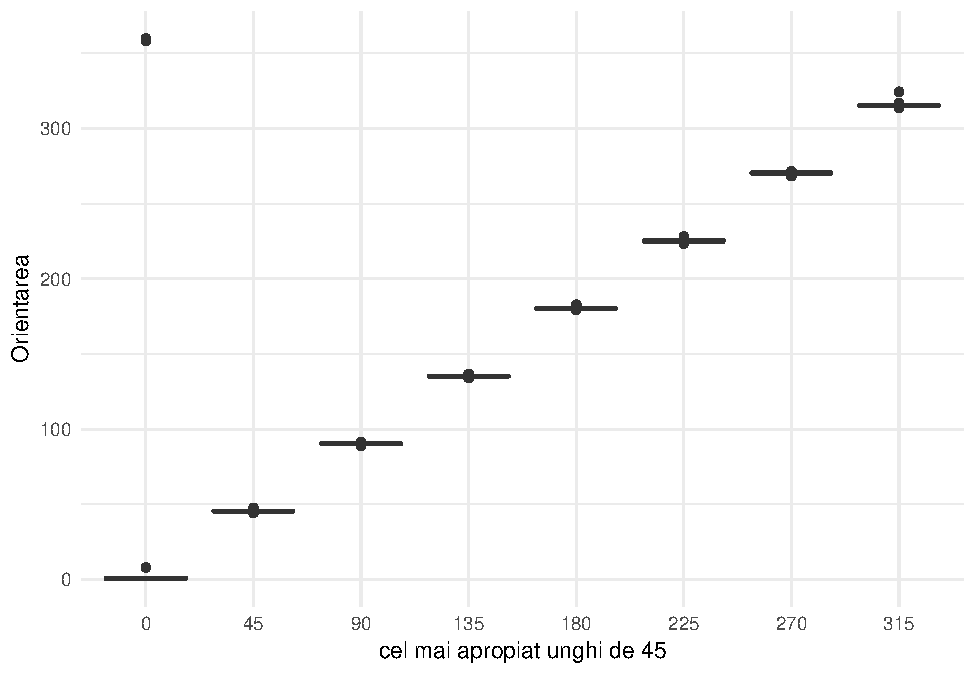
\includegraphics[width=0.9\linewidth]{Lab_1_2_files/figure-latex/unnamed-chunk-19-1} \end{center}

Testarea ipotezelor statistice cu ajutorul testului t-student (corecția
lui \texttt{Welch}):

\begin{Shaded}
\begin{Highlighting}[]
\KeywordTok{t.test}\NormalTok{(tempB, tempF) }\CommentTok{# Welch correction }
\end{Highlighting}
\end{Shaded}

\begin{verbatim}
## 
##  Welch Two Sample t-test
## 
## data:  tempB and tempF
## t = -2.2854, df = 127.51, p-value = 0.02394
## alternative hypothesis: true difference in means is not equal to 0
## 95 percent confidence interval:
##  -0.29980476 -0.02156277
## sample estimates:
## mean of x mean of y 
##  36.72479  36.88547
\end{verbatim}

Verificăm dacă cele două eșantioane au varianțe egale (folosim testul
lui \texttt{Fisher}):

\begin{Shaded}
\begin{Highlighting}[]
\KeywordTok{var.test}\NormalTok{(tempB, tempF)}
\end{Highlighting}
\end{Shaded}

\begin{verbatim}
## 
##  F test to compare two variances
## 
## data:  tempB and tempF
## F = 0.88329, num df = 64, denom df = 64, p-value = 0.6211
## alternative hypothesis: true ratio of variances is not equal to 1
## 95 percent confidence interval:
##  0.5387604 1.4481404
## sample estimates:
## ratio of variances 
##          0.8832897
\end{verbatim}

Aplicăm acum testul t-student cu opțiunea de varianțe egale
(\texttt{pooled\ variance}):

\begin{Shaded}
\begin{Highlighting}[]
\KeywordTok{t.test}\NormalTok{(tempB, tempF, }\DataTypeTok{var.equal =} \NormalTok{T) }\CommentTok{# without Welch correction }
\end{Highlighting}
\end{Shaded}

\begin{verbatim}
## 
##  Two Sample t-test
## 
## data:  tempB and tempF
## t = -2.2854, df = 128, p-value = 0.02393
## alternative hypothesis: true difference in means is not equal to 0
## 95 percent confidence interval:
##  -0.29979966 -0.02156786
## sample estimates:
## mean of x mean of y 
##  36.72479  36.88547
\end{verbatim}

\subsection{Exemplul 2}\label{exemplul-2}

\begin{Shaded}
\begin{Highlighting}[]
\CommentTok{# Example data}
\NormalTok{x <-}\StringTok{ }\KeywordTok{c}\NormalTok{(}\FloatTok{102.5}\NormalTok{, }\FloatTok{106.6}\NormalTok{,  }\FloatTok{99.8}\NormalTok{, }\FloatTok{106.5}\NormalTok{, }\FloatTok{103.7}\NormalTok{, }\FloatTok{105.5}\NormalTok{, }\FloatTok{98.2}\NormalTok{, }\FloatTok{104.1}\NormalTok{,  }\FloatTok{85.6}\NormalTok{, }\FloatTok{105.5}\NormalTok{, }\FloatTok{114.0}\NormalTok{, }\FloatTok{112.2}\NormalTok{)}
\NormalTok{y <-}\StringTok{ }\KeywordTok{c}\NormalTok{( }\FloatTok{93.7}\NormalTok{,  }\FloatTok{90.9}\NormalTok{, }\FloatTok{100.4}\NormalTok{,  }\FloatTok{92.0}\NormalTok{, }\FloatTok{100.2}\NormalTok{, }\FloatTok{104.6}\NormalTok{, }\FloatTok{95.4}\NormalTok{,  }\FloatTok{96.6}\NormalTok{,  }\FloatTok{99.2}\NormalTok{)}

\CommentTok{# Two-sided t-test allowing un-equal population SDs}
\KeywordTok{t.test}\NormalTok{(x,y)}
\end{Highlighting}
\end{Shaded}

\begin{verbatim}
## 
##  Welch Two Sample t-test
## 
## data:  x and y
## t = 2.6041, df = 18.475, p-value = 0.01769
## alternative hypothesis: true difference in means is not equal to 0
## 95 percent confidence interval:
##   1.30124 12.06543
## sample estimates:
## mean of x mean of y 
##  103.6833   97.0000
\end{verbatim}

\begin{Shaded}
\begin{Highlighting}[]
\KeywordTok{dotplot}\NormalTok{(x,y)}
\end{Highlighting}
\end{Shaded}

\begin{center}\includegraphics[width=0.9\linewidth]{Lab_1_2_files/figure-latex/unnamed-chunk-23-1} \end{center}

\subsection{Exemplul 3}\label{exemplul-3}

\begin{Shaded}
\begin{Highlighting}[]
\CommentTok{# One-tailed test example}
\NormalTok{x <-}\StringTok{ }\KeywordTok{c}\NormalTok{(}\FloatTok{59.4}\NormalTok{, }\FloatTok{52.3}\NormalTok{, }\FloatTok{42.6}\NormalTok{, }\FloatTok{45.1}\NormalTok{, }\FloatTok{65.9}\NormalTok{, }\FloatTok{40.8}\NormalTok{)}
\NormalTok{y <-}\StringTok{ }\KeywordTok{c}\NormalTok{(}\FloatTok{82.7}\NormalTok{, }\FloatTok{56.7}\NormalTok{, }\FloatTok{46.9}\NormalTok{, }\FloatTok{67.8}\NormalTok{, }\FloatTok{74.8}\NormalTok{, }\FloatTok{85.7}\NormalTok{)}

\CommentTok{# One-tailed t-test}
\KeywordTok{t.test}\NormalTok{(x,y,}\DataTypeTok{alt=}\StringTok{"less"}\NormalTok{)}
\end{Highlighting}
\end{Shaded}

\begin{verbatim}
## 
##  Welch Two Sample t-test
## 
## data:  x and y
## t = -2.4421, df = 8.6937, p-value = 0.01907
## alternative hypothesis: true difference in means is less than 0
## 95 percent confidence interval:
##       -Inf -4.454703
## sample estimates:
## mean of x mean of y 
##  51.01667  69.10000
\end{verbatim}

\begin{Shaded}
\begin{Highlighting}[]
\CommentTok{# The dotplot}
\KeywordTok{dotplot}\NormalTok{(x,y)}
\end{Highlighting}
\end{Shaded}

\begin{center}\includegraphics[width=0.9\linewidth]{Lab_1_2_files/figure-latex/unnamed-chunk-24-1} \end{center}

\subsection{Exemplul 4}\label{exemplul-4}

\begin{Shaded}
\begin{Highlighting}[]
\CommentTok{# another one-tailed test example}
\NormalTok{x <-}\StringTok{ }\KeywordTok{c}\NormalTok{(}\FloatTok{63.3}\NormalTok{, }\FloatTok{58.6}\NormalTok{, }\FloatTok{59.0}\NormalTok{, }\FloatTok{60.5}\NormalTok{, }\FloatTok{56.3}\NormalTok{, }\FloatTok{57.4}\NormalTok{)}
\NormalTok{y <-}\StringTok{ }\KeywordTok{c}\NormalTok{(}\FloatTok{75.6}\NormalTok{, }\FloatTok{65.9}\NormalTok{, }\FloatTok{72.3}\NormalTok{, }\FloatTok{58.0}\NormalTok{, }\FloatTok{64.4}\NormalTok{, }\FloatTok{66.2}\NormalTok{)}
\KeywordTok{t.test}\NormalTok{(x,y,}\DataTypeTok{alt=}\StringTok{"less"}\NormalTok{)}
\end{Highlighting}
\end{Shaded}

\begin{verbatim}
## 
##  Welch Two Sample t-test
## 
## data:  x and y
## t = -2.8968, df = 6.5546, p-value = 0.01242
## alternative hypothesis: true difference in means is less than 0
## 95 percent confidence interval:
##       -Inf -2.674212
## sample estimates:
## mean of x mean of y 
##  59.18333  67.06667
\end{verbatim}

\begin{Shaded}
\begin{Highlighting}[]
\KeywordTok{dotplot}\NormalTok{(x,y)}
\end{Highlighting}
\end{Shaded}

\begin{center}\includegraphics[width=0.9\linewidth]{Lab_1_2_files/figure-latex/unnamed-chunk-25-1} \end{center}

\subsection{Grafic recomandat}\label{grafic-recomandat}

\begin{Shaded}
\begin{Highlighting}[]
\NormalTok{x <-}\StringTok{ }\KeywordTok{c}\NormalTok{(}\FloatTok{15.1}\NormalTok{, }\FloatTok{13.1}\NormalTok{, }\FloatTok{21.5}\NormalTok{)}
\NormalTok{y <-}\StringTok{ }\KeywordTok{c}\NormalTok{(}\FloatTok{35.1}\NormalTok{, }\FloatTok{39.5}\NormalTok{, }\FloatTok{58.8}\NormalTok{)}

\KeywordTok{par}\NormalTok{(}\DataTypeTok{mar=}\KeywordTok{c}\NormalTok{(}\DecValTok{4}\NormalTok{,}\DecValTok{4}\NormalTok{,}\DecValTok{2}\NormalTok{,}\DecValTok{1}\NormalTok{),}\DataTypeTok{mfrow=}\KeywordTok{c}\NormalTok{(}\DecValTok{1}\NormalTok{,}\DecValTok{2}\NormalTok{),}\DataTypeTok{las=}\DecValTok{1}\NormalTok{)}

\KeywordTok{barplot}\NormalTok{(}\KeywordTok{c}\NormalTok{(}\KeywordTok{mean}\NormalTok{(x),}\KeywordTok{mean}\NormalTok{(y)),}\DataTypeTok{width=}\DecValTok{1}\NormalTok{,}\DataTypeTok{space=}\KeywordTok{c}\NormalTok{(}\FloatTok{0.5}\NormalTok{,}\FloatTok{0.5}\NormalTok{),}
        \DataTypeTok{col=}\KeywordTok{c}\NormalTok{(}\StringTok{"white"}\NormalTok{,}\StringTok{"gray40"}\NormalTok{),}\DataTypeTok{xlim=}\KeywordTok{c}\NormalTok{(}\DecValTok{0}\NormalTok{,}\DecValTok{3}\NormalTok{),}\DataTypeTok{names=}\KeywordTok{c}\NormalTok{(}\StringTok{"A"}\NormalTok{,}\StringTok{"B"}\NormalTok{),}
        \DataTypeTok{ylim=}\KeywordTok{c}\NormalTok{(}\DecValTok{0}\NormalTok{,}\DecValTok{76}\NormalTok{))}
\KeywordTok{segments}\NormalTok{(}\DecValTok{1}\NormalTok{,}\KeywordTok{mean}\NormalTok{(x),}\DecValTok{1}\NormalTok{,}\KeywordTok{mean}\NormalTok{(x)+}\KeywordTok{sd}\NormalTok{(x),}\DataTypeTok{lwd=}\DecValTok{2}\NormalTok{)}
\KeywordTok{segments}\NormalTok{(}\FloatTok{0.8}\NormalTok{,}\KeywordTok{mean}\NormalTok{(x)+}\KeywordTok{sd}\NormalTok{(x),}\FloatTok{1.2}\NormalTok{,}\KeywordTok{mean}\NormalTok{(x)+}\KeywordTok{sd}\NormalTok{(x),}\DataTypeTok{lwd=}\DecValTok{2}\NormalTok{)}
\KeywordTok{segments}\NormalTok{(}\FloatTok{2.5}\NormalTok{,}\KeywordTok{mean}\NormalTok{(y),}\FloatTok{2.5}\NormalTok{,}\KeywordTok{mean}\NormalTok{(y)+}\KeywordTok{sd}\NormalTok{(y),}\DataTypeTok{lwd=}\DecValTok{2}\NormalTok{)}
\KeywordTok{segments}\NormalTok{(}\FloatTok{2.3}\NormalTok{,}\KeywordTok{mean}\NormalTok{(y)+}\KeywordTok{sd}\NormalTok{(y),}\FloatTok{2.7}\NormalTok{,}\KeywordTok{mean}\NormalTok{(y)+}\KeywordTok{sd}\NormalTok{(y),}\DataTypeTok{lwd=}\DecValTok{2}\NormalTok{)}
\KeywordTok{mtext}\NormalTok{(}\StringTok{"Grafic nepotrivit"}\NormalTok{,}\DataTypeTok{cex=}\FloatTok{1.5}\NormalTok{,}\DataTypeTok{line=}\FloatTok{0.5}\NormalTok{)}

\KeywordTok{plot}\NormalTok{(}\KeywordTok{rep}\NormalTok{(}\DecValTok{0}\NormalTok{:}\DecValTok{1}\NormalTok{,}\KeywordTok{c}\NormalTok{(}\DecValTok{3}\NormalTok{,}\DecValTok{3}\NormalTok{)),}\KeywordTok{c}\NormalTok{(x,y),}\DataTypeTok{xaxt=}\StringTok{"n"}\NormalTok{,}\DataTypeTok{ylim=}\KeywordTok{c}\NormalTok{(}\DecValTok{0}\NormalTok{,}\DecValTok{76}\NormalTok{),}
     \DataTypeTok{xlim=}\KeywordTok{c}\NormalTok{(-}\FloatTok{0.5}\NormalTok{,}\FloatTok{1.5}\NormalTok{),}\DataTypeTok{ylab=}\StringTok{""}\NormalTok{,}\DataTypeTok{xlab=}\StringTok{""}\NormalTok{)}
\KeywordTok{abline}\NormalTok{(}\DataTypeTok{v=}\DecValTok{0}\NormalTok{:}\DecValTok{1}\NormalTok{,}\DataTypeTok{col=}\StringTok{"gray40"}\NormalTok{,}\DataTypeTok{lty=}\DecValTok{2}\NormalTok{)}
\KeywordTok{points}\NormalTok{(}\KeywordTok{rep}\NormalTok{(}\DecValTok{0}\NormalTok{:}\DecValTok{1}\NormalTok{,}\KeywordTok{c}\NormalTok{(}\DecValTok{3}\NormalTok{,}\DecValTok{3}\NormalTok{)),}\KeywordTok{c}\NormalTok{(x,y),}\DataTypeTok{lwd=}\DecValTok{2}\NormalTok{)}
\KeywordTok{mtext}\NormalTok{(}\StringTok{"Grafic recomandat"}\NormalTok{,}\DataTypeTok{cex=}\FloatTok{1.5}\NormalTok{,}\DataTypeTok{line=}\FloatTok{0.5}\NormalTok{)}
\NormalTok{xci <-}\StringTok{ }\KeywordTok{t.test}\NormalTok{(x)$conf.int}
\NormalTok{yci <-}\StringTok{ }\KeywordTok{t.test}\NormalTok{(y)$conf.int}
\KeywordTok{segments}\NormalTok{(}\FloatTok{0.25}\NormalTok{,xci[}\DecValTok{1}\NormalTok{],}\FloatTok{0.25}\NormalTok{,xci[}\DecValTok{2}\NormalTok{],}\DataTypeTok{lwd=}\DecValTok{2}\NormalTok{,}\DataTypeTok{col=}\StringTok{"darkgray"}\NormalTok{)}
\KeywordTok{segments}\NormalTok{(}\KeywordTok{c}\NormalTok{(}\FloatTok{0.23}\NormalTok{,}\FloatTok{0.23}\NormalTok{,}\FloatTok{0.2}\NormalTok{),}\KeywordTok{c}\NormalTok{(xci,}\KeywordTok{mean}\NormalTok{(x)),}\KeywordTok{c}\NormalTok{(}\FloatTok{0.27}\NormalTok{,}\FloatTok{0.27}\NormalTok{,}\FloatTok{0.3}\NormalTok{),}
         \KeywordTok{c}\NormalTok{(xci,}\KeywordTok{mean}\NormalTok{(x)),}\DataTypeTok{lwd=}\DecValTok{2}\NormalTok{,}\DataTypeTok{col=}\StringTok{"darkgray"}\NormalTok{)}
\KeywordTok{segments}\NormalTok{(}\DecValTok{1}\FloatTok{-0.25}\NormalTok{,yci[}\DecValTok{1}\NormalTok{],}\DecValTok{1}\FloatTok{-0.25}\NormalTok{,yci[}\DecValTok{2}\NormalTok{],}\DataTypeTok{lwd=}\DecValTok{2}\NormalTok{,}\DataTypeTok{col=}\StringTok{"brown3"}\NormalTok{)}
\KeywordTok{segments}\NormalTok{(}\DecValTok{1}\NormalTok{-}\KeywordTok{c}\NormalTok{(}\FloatTok{0.23}\NormalTok{,}\FloatTok{0.23}\NormalTok{,}\FloatTok{0.2}\NormalTok{),}\KeywordTok{c}\NormalTok{(yci,}\KeywordTok{mean}\NormalTok{(y)),}\DecValTok{1}\NormalTok{-}\KeywordTok{c}\NormalTok{(}\FloatTok{0.27}\NormalTok{,}\FloatTok{0.27}\NormalTok{,}\FloatTok{0.3}\NormalTok{),}
         \KeywordTok{c}\NormalTok{(yci,}\KeywordTok{mean}\NormalTok{(y)),}\DataTypeTok{lwd=}\DecValTok{2}\NormalTok{,}\DataTypeTok{col=}\StringTok{"brown3"}\NormalTok{)}
\NormalTok{u <-}\StringTok{ }\KeywordTok{par}\NormalTok{(}\StringTok{"usr"}\NormalTok{)}
\KeywordTok{segments}\NormalTok{(}\DecValTok{0}\NormalTok{:}\DecValTok{1}\NormalTok{,u[}\DecValTok{3}\NormalTok{],}\DecValTok{0}\NormalTok{:}\DecValTok{1}\NormalTok{,u[}\DecValTok{3}\NormalTok{]-}\KeywordTok{diff}\NormalTok{(u[}\DecValTok{3}\NormalTok{:}\DecValTok{4}\NormalTok{])*}\FloatTok{0.03}\NormalTok{,}\DataTypeTok{xpd=}\OtherTok{TRUE}\NormalTok{)}
\KeywordTok{text}\NormalTok{(}\DecValTok{0}\NormalTok{:}\DecValTok{1}\NormalTok{,u[}\DecValTok{3}\NormalTok{]-}\KeywordTok{diff}\NormalTok{(u[}\DecValTok{3}\NormalTok{:}\DecValTok{4}\NormalTok{])*}\FloatTok{0.08}\NormalTok{,}\KeywordTok{c}\NormalTok{(}\StringTok{"A"}\NormalTok{,}\StringTok{"B"}\NormalTok{),}\DataTypeTok{xpd=}\OtherTok{TRUE}\NormalTok{)}
\end{Highlighting}
\end{Shaded}

\begin{center}\includegraphics[width=0.9\linewidth]{Lab_1_2_files/figure-latex/unnamed-chunk-26-1} \end{center}

\section{Testarea ipotezelor statistice: inferență asupra a două
eșantioane dependente
(perechi)}\label{testarea-ipotezelor-statistice-inferenta-asupra-a-doua-esantioane-dependente-perechi}

\begin{center}\rule{0.5\linewidth}{\linethickness}\end{center}

Considerăm următorul set de date din pachetul \texttt{MASS} (luarea in
greutate de catre femei anorexice):

\begin{Shaded}
\begin{Highlighting}[]
\KeywordTok{data}\NormalTok{(anorexia, }\DataTypeTok{package=}\StringTok{"MASS"}\NormalTok{)      }
\KeywordTok{attach}\NormalTok{(anorexia)}
\KeywordTok{str}\NormalTok{(anorexia)}
\end{Highlighting}
\end{Shaded}

\begin{verbatim}
## 'data.frame':    72 obs. of  3 variables:
##  $ Treat : Factor w/ 3 levels "CBT","Cont","FT": 2 2 2 2 2 2 2 2 2 2 ...
##  $ Prewt : num  80.7 89.4 91.8 74 78.1 88.3 87.3 75.1 80.6 78.4 ...
##  $ Postwt: num  80.2 80.1 86.4 86.3 76.1 78.1 75.1 86.7 73.5 84.6 ...
\end{verbatim}

\begin{Shaded}
\begin{Highlighting}[]
\NormalTok{ft=}\KeywordTok{subset}\NormalTok{(anorexia,}\DataTypeTok{Treat=}\StringTok{"FT"}\NormalTok{) }\CommentTok{# family treatment}
\end{Highlighting}
\end{Shaded}

Testăm dacă există diferențe între luarea în greutate înainte de
tratament și după tratament:

\begin{Shaded}
\begin{Highlighting}[]
\KeywordTok{with}\NormalTok{(ft, }\KeywordTok{t.test}\NormalTok{(Postwt-Prewt, }\DataTypeTok{mu=}\DecValTok{0}\NormalTok{, }\DataTypeTok{alternative=}\StringTok{"greater"}\NormalTok{))}
\end{Highlighting}
\end{Shaded}

\begin{verbatim}
## 
##  One Sample t-test
## 
## data:  Postwt - Prewt
## t = 2.9376, df = 71, p-value = 0.002229
## alternative hypothesis: true mean is greater than 0
## 95 percent confidence interval:
##  1.195825      Inf
## sample estimates:
## mean of x 
##  2.763889
\end{verbatim}

sau

\begin{Shaded}
\begin{Highlighting}[]
\KeywordTok{with}\NormalTok{(ft, }\KeywordTok{t.test}\NormalTok{(Postwt, Prewt, }\DataTypeTok{paired=}\NormalTok{T, }\DataTypeTok{alternative=}\StringTok{"greater"}\NormalTok{))}
\end{Highlighting}
\end{Shaded}

\begin{verbatim}
## 
##  Paired t-test
## 
## data:  Postwt and Prewt
## t = 2.9376, df = 71, p-value = 0.002229
## alternative hypothesis: true difference in means is greater than 0
## 95 percent confidence interval:
##  1.195825      Inf
## sample estimates:
## mean of the differences 
##                2.763889
\end{verbatim}


\end{document}
